\documentclass{article}

\usepackage[english]{babel}
\usepackage[utf8x]{inputenc}
\usepackage{amsmath}
\usepackage{amssymb}
\usepackage{graphicx}
\graphicspath{{./}}
\begin{document}

Ivan Lin

Dr. Michael Bender

CSE150 - Honors Foundations of Computer Science Fall 2016

\begin{center}
Homework 3a
\end{center}

\underline{Problem 2}

Show that every subset of $\mathbb{N}$ is countable.

\underline{Proof}

Let $f: X\implies {N}$, where $f(x)=min\{\mathbb{N}-\cup_{i=0}^{x-1}f(i)$, or for each $x$, $f(x)$ returns the smallest number in the set of natural numbers not given to a lower value of $x$.

\underline{Problem 3}

Show that the set of all integers ($\mathbb{Z}$) is countable.

\underline{Proof}

We will show $\mathbb{Z}$ is countable by proving a bijection between $\mathbb{Z}$ and $\mathbb{N}$.

Let $f: \mathbb{Z} \implies \mathbb{N}$, where $f(n)=2n$ if $n \geq 0$, $-2n+1$ if $n \leq 0$

$f$ is one to one. If $f(a)=f(b)$ for some $a,b\in X$ and $f(a),f(b)$ is even, then $f(a)=2a=f(b)=2b$. If $f(a),f(b)$ is odd, then $f(a)=-2a+1=f(b)=-2b+1$. In either case, the equation simplifies to $a=b$, meaning the only time two inputs produce the same output is when they are equal.

$f$ is onto. We need to show that $\forall n \in \mathbb{N}, \exists z \in \mathbb{Z}, f(z)=n$. Let $z=\frac{n}{2}$ if $n$ is even, $-\frac{n-1}{2}$ if $n$ is odd

$f(\frac{n}{2})=2*\frac{n}{2}=n$ where $n$ is odd, $f(-\frac{n-1}{2})=-\frac{n-1}{2}+1$ where $n$ is even

Since $\frac{n}{2}\in \mathbb{N}$ when $n$ is even and natural, $\frac{n-1}{2}\in mathbb{N}$ where $n$ is an odd normal, the union of the domains cover all $\mathbb{N}$ and the range cover all $\mathbb{N}$.

Since there exists a bijection between $\mathbb{Z}$ and $\mathbb{N}$, $\mathbb{Z}$ is countable.

\underline{Problem 4}

Show that all \textit{finite} subsets of a countable set are countable.

\underline{Proof}

We will prove that all finite subsets of a countable set are countable by proving all finite sets are countable.

Let $S$ be a finite set where every element is denoted $s_n$ where $n$ is a finite index in $S$ less than n.

Let $f$ be a function $f(s_n)=n, n\in \mathbb{N}, n[0,n)$.

Since every element $s_n$ is indexed by a natural number, every element in $s$ maps to a natural number, implying $S$ is countable.

\underline{Problem 5}

Show that the following statements are equivalent and true (Statements $P$ and $Q$ are \textit{equivalent} if $P \iff Q$):
\begin{itemize}
\item $\mathbb{N}\times\mathbb{N}$ is countable
\item Union of countably many countable sets is countable
\item $\mathbb{Q}$ is countable
\end{itemize}

\underline{Proof}

We will show $\mathbb{N}\times\mathbb{N}$ is countable.

Let $f: \mathbb{N}^2 \implies \mathbb{N}$, where $f(x,y) = y + \sum_{i=0}^{x + y + 1}i$

This function maps to a path shown below.

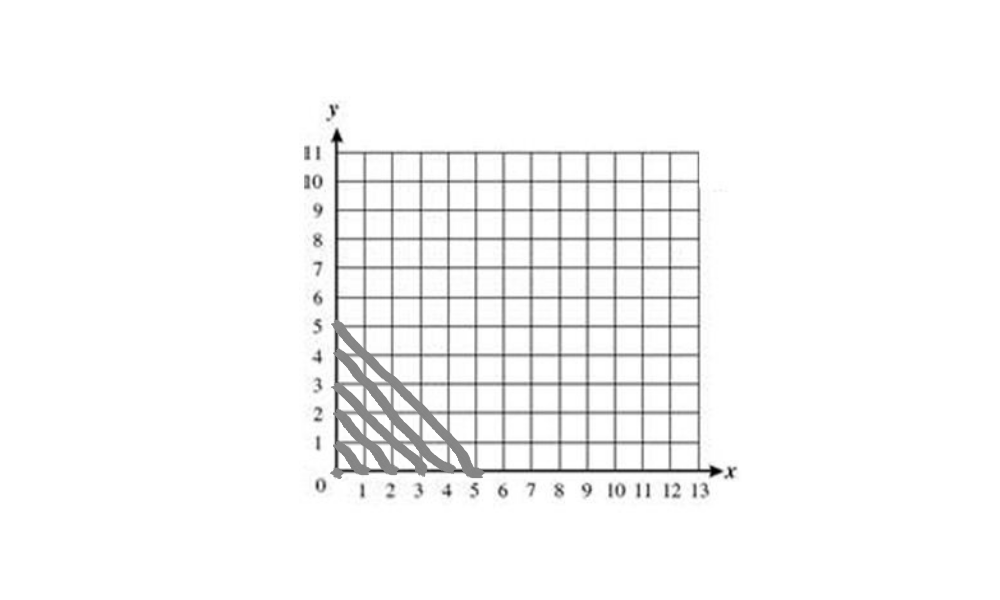
\includegraphics[width=8cm, height=5cm]{q5graph}

This graph shows that the function is one-to-one, or that if $f(x,y)=f(a,b)$, then $(x,y)=(a,b)$.

This maps every possible $(\mathbb{N},\mathbb{N})$ to a natural number, therefore $\mathbb{N}\times\mathbb{N}$ is countable.

\bigskip

We will show the union of countable many countable sets is countable.

Any countable set can be mapped to a natural number. 

Let set $S$ be the set containing a countable number of countable subsets, each denoted $S_n$. 

Let $f$ map an element in index $m$ of any $S_n$ to a natural number.

Let $f: \mathbb{N}^2 \implies \mathbb{N}$, where $f(n,m) = m + \sum_{i=0}^{n + m + 1}i$

The function is one-to-one, meaning that if $f(n,m)=f(a,b)$, then $(n,m)=(a,b)$.

This maps every element $S_{n,m}$ to a natural number, therefore the union of a countable number of countable sets is countable.

\bigskip

We will show that $\mathbb{Q}$ is countable.

Any distinct rational number $q\in Q$ can be written as a quotient of a distinct pair of natural numbers $q=\frac{a}{b},a,b\in\mathbb{N}$.

Let $f:(a,b)\implies\mathbb{N}$, where $f(a,b) = m + \sum_{i=0}^{n + m + 1}i$.

This maps the pair $(a,b)$ to a natural number, which means the pair is countable.

The function is ome-to-one, meaning that if $f(n,m)=f(a,b)$, then $(n,m)=(a,b)$.

Since $\mathbb{Q}\implies (a,b)\implies \mathbb{N}$, the set of rational numbers $Q$ is countable.

\underline{Problem 6}

A submarine is moving along the integer number line at a constant speed $s$ so that at each hour it is on an
integer number. It started moving at time 0 at some position $b$. If $t$ is the (whole) number of hours elapsed
since the submarine started moving, then its position is given by the equation $x = st + b$, where $x$, $s$ and $b$
are integers.
\smallskip
You are working at Rocket Pizza delivery and you are to deliver pizza to the submarine. At each hour you
can drop pizza on any number on the integer line. If the submarine is there at that time, then you have
delivered the pizza and your job is done (you will be notified as soon as it happens).
\smallskip
The problem is that you don’t know where the submarine is, you cannot see it, you don’t know where it
started and how fast it is moving (i.e., you don’t know values of $s$ and $b$ - classified top secret data). The
upside is that you have infinite number of pizzas.
\smallskip
Show that you can deliver pizza in a finite amount of time.
\bigskip

$s$ is an integer and $b$ is an integer. The set of all possible combinations of two countably infinite sets, $\mathbb{Z}\times\mathbb{Z}$, is also countable. Given that you know $t$ and $\mathbb{Z}\times\mathbb{Z}$ is countable, you can select a $(s,b)$ every hour to apply to the equation to get an $x$ to drop the pizza. Eventually this will yield an $x$ that the submarine is at.

\underline{Problem 7} 

In the following table, F stands for Finite, I for Infinitely Countable, C for Countable, U for uncountable. Put a checkmark next
to the strongest statement you can make about the resulting set (i.e. correct answer for $F \cup F$ is finite, even though it is 
countable as well). Check \textbf{?} whenever there's not enough information to decide, i.e. there can be different cases with 
no `strongest' answer.

\bigskip

\begin{center}
\begin{tabular}{c|c|c|c|c|c|c|c|c|c|c|c|c} \hline
Set & F & I & C & U & ? & $\star$ & Set & F & I & C & U & ?  \\ \hline

$F \cup F$ & \checkmark & & & & & $\star$ & $C \cup F$ & & & \checkmark & & \\ \hline
$F \cup I$ & & \checkmark & & & & $\star$ & $C \cup I$ & & & \checkmark & & \\ \hline
$F \cup C$ & & & \checkmark & & & $\star$ & $C \cup C$ & & & \checkmark & & \\ \hline
$F \cup U$ & & & & \checkmark & & $\star$ & $C \cup U$ & & & & \checkmark & \\ \hline
$F \cap F$ & \checkmark & & & & & $\star$ & $C \cap F$ & \checkmark & & & & \\ \hline
$F \cap I$ & \checkmark & & & & & $\star$ & $C \cap I$ & & & \checkmark & & \\ \hline
$F \cap C$ & \checkmark & & & & & $\star$ & $C \cap C$ & & & \checkmark & & \\ \hline
$F \cap U$ & \checkmark & & & & & $\star$ & $C \cap U$ & & & \checkmark & & \\ \hline
$F - F$ & \checkmark & & & & & $\star$ & $C - F$ & & & \checkmark & & \\ \hline
$F - I$ & \checkmark & & & & & $\star$ & $C - I$ & & & \checkmark & & \\ \hline
$F - C$ & \checkmark & & & & & $\star$ & $C - C$ & & & \checkmark & & \\ \hline
$F - U$ & \checkmark & & & & & $\star$ & $C - U$ & & & \checkmark & & \\ \hline
$F \times F$ & \checkmark & & & & & $\star$ & $C \times F$ & & & \checkmark & & \\ \hline
$F \times I$ & & \checkmark & & & & $\star$ & $C \times I$ & & & \checkmark & & \\ \hline
$F \times C$ & & & \checkmark & & & $\star$ & $C \times C$ & & & \checkmark & & \\ \hline
$F \times U$ & & & & \checkmark & & $\star$ & $C \times U$ & & & & \checkmark & \\ \hline
$I \cup F$ & & \checkmark & & & & $\star$ & $U \cup F$ & & & & \checkmark & \\ \hline
$I \cup I$ & & \checkmark & & & & $\star$ & $U \cup I$ & & & & \checkmark & \\ \hline
$I \cup C$ & & \checkmark & & & & $\star$ & $U \cup C$ & & & & \checkmark & \\ \hline
$I \cup U$ & & & & \checkmark & & $\star$ & $U \cup U$ & & & & \checkmark & \\ \hline
$I \cap F$ & \checkmark & & & & & $\star$ & $U \cap F$ & \checkmark & & & & \\ \hline
$I \cap I$ & & & \checkmark & & & $\star$ & $U \cap I$ & & \checkmark & & & \\ \hline
$I \cap C$ & & & \checkmark & & & $\star$ & $U \cap C$ & & & \checkmark & & \\ \hline
$I \cap U$ & & & \checkmark & & & $\star$ & $U \cap U$ & & & & & \checkmark \\ \hline
$I - F$ & & \checkmark & & & & $\star$ & $U - F$ & & & & \checkmark & \\ \hline
$I - I$ & & & \checkmark & & & $\star$ & $U - I$ & & & & \checkmark & \\ \hline
$I - C$ & & & \checkmark & & & $\star$ & $U - C$ & & & & \checkmark & \\ \hline
$I - U$ & & & \checkmark & & & $\star$ & $U - U$ & & & & & \checkmark \\ \hline
$I \times F$ & & \checkmark & & & & $\star$ & $U \times F$ & & & & \checkmark & \\ \hline
$I \times I$ & & \checkmark & & & & $\star$ & $U \times I$ & & & & \checkmark & \\ \hline
$I \times C$ & & \checkmark & & & & $\star$ & $U \times C$ & & & & \checkmark & \\ \hline
$I \times U$ & & & & \checkmark & & $\star$ & $U \times U$ & & & & \checkmark & \\ \hline
\end{tabular}
\end{center}


\end{document}
